% Article de vulgarisation, quatre pages A4 (un A3 plié). Compiler : cd docs/vulgarisation && tectonic -X compile article.tex
% L'imposition pour l'impression en A3 plié est dans livret-a3.tex.
\documentclass[10pt]{article}
\usepackage{fontspec}
\setmainfont{Charter}
\newfontfamily\titre{Avenir Next}[UprightFont=* Bold, BoldFont=* Heavy]
\newfontfamily\sans{Avenir Next}[UprightFont=* Regular, BoldFont=* Demi Bold, ItalicFont=* Italic]
\newfontfamily\sanscond{Avenir Next Condensed}[UprightFont=* Demi Bold]
\usepackage{polyglossia}\setmainlanguage{french}
\usepackage[a4paper,margin=14mm,top=13mm,bottom=14mm]{geometry}
\usepackage{multicol,graphicx,xcolor,tcolorbox,microtype,amssymb,needspace}
\usepackage[hidelinks]{hyperref}
\setlength{\columnsep}{5mm}
\setlength{\parindent}{1em}
\setlength{\parskip}{0pt}
\definecolor{bleu}{HTML}{38539D}
\definecolor{orange}{HTML}{E0612B}
\definecolor{encre}{HTML}{2B2A27}
\definecolor{gris}{HTML}{6F6B63}
\definecolor{papier}{HTML}{F4EFE6}
\pagestyle{empty}
\newcommand{\surtitre}[1]{{\sanscond\color{orange}\fontsize{11}{13}\selectfont\MakeUppercase{#1}}}
\newcommand{\inter}[1]{\par\needspace{5\baselineskip}\medskip{\sans\bfseries\color{bleu}\fontsize{11}{13}\selectfont #1}\par\nobreak\smallskip\noindent\ignorespaces}
\newcommand{\legende}[1]{{\sans\fontsize{8}{10}\selectfont\color{gris}#1}}
\newcommand{\exergue}[1]{\par\medskip{\titre\color{orange}\fontsize{14}{17}\selectfont «\,#1\,»}\par\medskip}
\newtcolorbox{encadre}[1]{colback=papier,colframe=papier,arc=0pt,boxrule=0pt,left=3mm,right=3mm,top=2.5mm,bottom=2.5mm,fontupper=\sans\fontsize{8.6}{11}\selectfont,title={\sans\bfseries\fontsize{10.5}{12}\selectfont\color{orange}#1},coltitle=orange,colbacktitle=papier,toptitle=1mm}
\newcommand{\folio}[1]{\vfill\noindent{\sans\fontsize{7.5}{9}\selectfont\color{gris}Les cartons secrets de Grothendieck\hfill #1}}
\fontsize{9.6}{12.4}\selectfont

\begin{document}

% ------------------------------------------------------------- page 1
\noindent\surtitre{Mathématiques · Archives}\par\vspace{4mm}
\noindent{\titre\color{encre}\fontsize{46}{48}\selectfont Les cartons secrets\\[1mm] de Grothendieck}\par\vspace{5mm}
\noindent\begin{minipage}{0.86\textwidth}
{\sans\fontsize{13.5}{18}\selectfont\color{encre}En 1970, l'un des mathématiciens les plus influents du XX\textsuperscript{e} siècle quitte la recherche officielle. Il n'a pourtant jamais cessé d'écrire. Seize mille pages de ses brouillons dorment à Montpellier, vingt-deux mille feuillets à la Bibliothèque nationale. Une machine les a lus. Voici ce qu'elle y a trouvé, et ce qu'elle a manqué.}
\end{minipage}\par\vspace{3mm}
\noindent{\sans\fontsize{8.5}{10}\selectfont\color{gris}Par Michel Hua}\par\vspace{5mm}

\begin{multicols}{3}
\noindent{\titre\fontsize{30}{30}\selectfont\color{bleu}D}ans les années 1960, Alexandre Grothendieck a refait de fond en comble la géométrie algébrique, cette branche des mathématiques qui étudie les figures définies par des équations. Ses traités, les EGA et les SGA, comptent ensemble environ huit mille pages imprimées ; on y apprend encore aujourd'hui. Médaille Fields en 1966, il quitte en 1970 l'Institut des hautes études scientifiques, rompt avec le milieu, s'installe dans le Sud de la France et finit sa vie retiré dans un village des Pyrénées, où il meurt en 2014.

On a longtemps cru qu'après 1970 il avait plus ou moins arrêté les mathématiques. Ses papiers racontent autre chose. En 1990 et 1995, il confie ses manuscrits mathématiques à Jean Malgoire, un ancien élève. Déposés à l'université de Montpellier en 2010, donnés en 2012, ils sont aujourd'hui en libre accès : 178 dossiers, 16\,074 pages numérisées. Le reste, ses écrits des années 1987 à 1999, est entré à la BnF : 43 boîtes, 22\,495 feuillets.

\inter{Des brouillons sans date}
Le problème, c'est que presque personne ne les a lus. Une vingtaine de dossiers ont été édités à la main par des mathématiciens, dont les célèbres \emph{Dérivateurs} et le premier volume d'\emph{À la poursuite des champs}. Les autres sont des notes de travail à l'encre et au crayon, reprises, raturées, annotées, dans une notation qui lui est propre. Et elles ne sont presque jamais datées : sur 164 dossiers transcrits, Grothendieck n'a daté ses feuillets de sa main que dans vingt et un. Les dates de l'inventaire sont pour la plupart déduites par les archivistes, d'après un verso, une lettre ou un dossier voisin.

\inter{Une machine en première lecture}
Depuis août 2026, un modèle de langage sert de premier lecteur. Il transcrit les dossiers par lots de vingt pages, en marquant ce qu'il a lu avec certitude, ce qu'il a deviné et ce qui reste illisible. Puis il rédige pour chaque dossier une lecture « modernisée », qui reformule les mathématiques dans les notations d'aujourd'hui. À ce jour, 165 dossiers sont transcrits.

Une troisième étape cherche dans la littérature les énoncés qui pourraient être nouveaux. Le registre en compte 456 ; pour 83 d'entre eux, la recherche a montré qu'ils étaient déjà imprimés, souvent bien plus tard, parfois sous la plume de Grothendieck lui-même.

\begin{encadre}{En chiffres}
\textbf{178} dossiers à Montpellier, \textbf{16\,074} pages\\[1pt]
\textbf{43} boîtes à la BnF, \textbf{22\,495} feuillets\\[1pt]
\textbf{21} dossiers seulement datés de sa main, sur 164\\[1pt]
\textbf{456} énoncés recensés, dont \textbf{83} retrouvés dans la littérature\\[1pt]
plus de \textbf{2\,000} théorèmes vérifiés par ordinateur\\[1pt]
\textbf{14} problèmes ouverts confiés aux mathématiciens
\end{encadre}

Reste à savoir si ces énoncés sont justes. Pour cela, l'édition utilise Lean, un logiciel qui vérifie une démonstration pas à pas, sans rien laisser passer. Plus de deux mille théorèmes tirés des dossiers y ont été démontrés. Lean a aussi servi de détecteur d'erreurs : il a trouvé des lectures fautives de la machine, des glissements dans les pages elles-mêmes, et quelques affirmations de Grothendieck qui sont fausses telles qu'il les a écrites.
\end{multicols}
\folio{1}
\newpage

% ------------------------------------------------------------- page 2
\noindent\begin{minipage}[t]{\textwidth}
\centering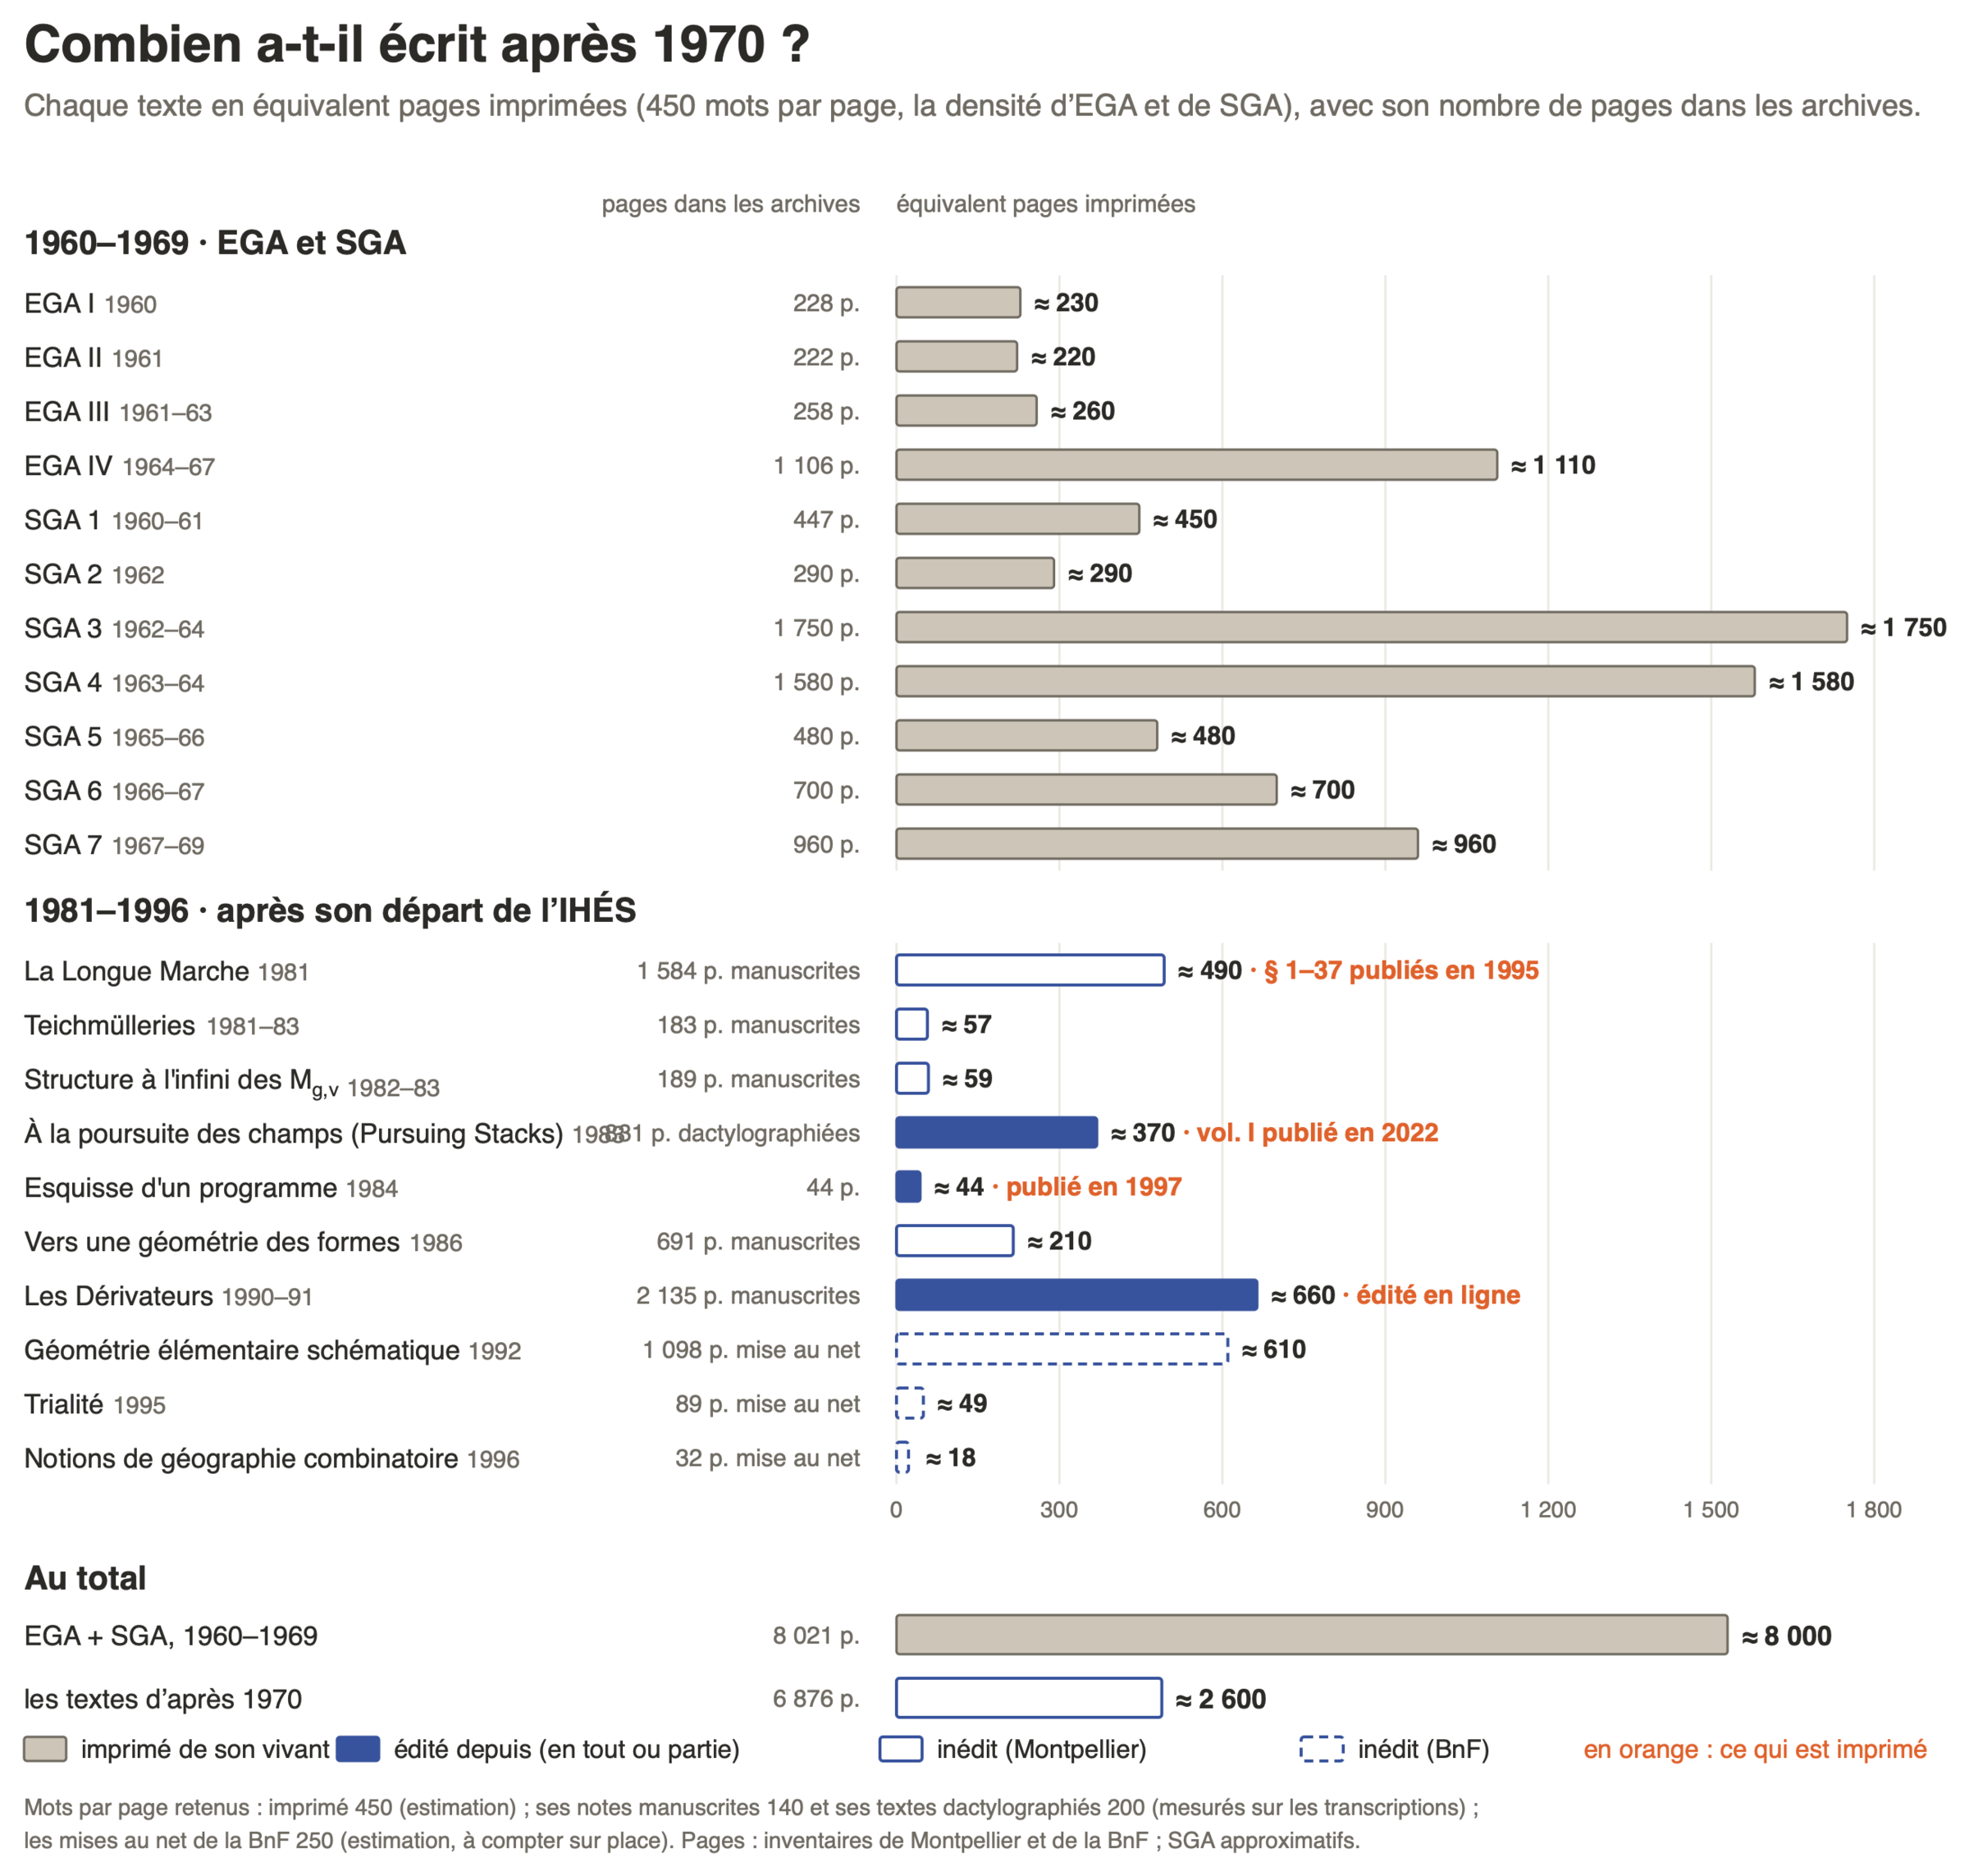
\includegraphics[height=0.43\textheight]{fig/later-writing-fr.png}\par\vspace{1mm}\raggedright
\legende{\textbf{Il n'a jamais arrêté.} Chaque texte est mesuré en équivalent pages imprimées, à 450 mots par page comme dans les EGA et SGA, pour comparer des manuscrits de densités différentes. Les longs textes écrits après son départ représentent environ un tiers des traités des années 1960. Les densités des mises au net de la BnF sont estimées ; elles seront mesurées sur place.}
\end{minipage}\par\vspace{4mm}

\begin{multicols}{3}
\inter{Après 1970, une œuvre souterraine}
Le premier constat est simple : il a continué. \emph{La Longue Marche à travers la théorie de Galois} (1981) fait près de 1\,600 pages manuscrites. \emph{À la poursuite des champs} (1983), tapé à la machine, en compte plus de 800. \emph{Les Dérivateurs} (1990--1991), plus de 2\,100. Entre les deux, des textes restés inconnus du public, comme les \emph{Teichmülleries} ou \emph{Vers une géométrie des formes}, écrit en juin et juillet 1986, où il cherche une géométrie sans points, faite de morceaux et de leurs contacts. L'idée n'est pas neuve chez lui : les topos qu'il avait inventés dans les années 1960 n'ont déjà pas besoin de points pour exister.

Les cartons de la BnF prolongent l'histoire jusqu'en 1999, mais changent de nature. L'essentiel est une méditation philosophique et spirituelle, \emph{La Clef des Songes} puis \emph{Le Problème du Mal}, sur des milliers de feuillets. Les mathématiques n'y reviennent que par épisodes : une \emph{Géométrie élémentaire schématique} de 1992, d'une écriture soignée, une \emph{Trialité} en 1995, des \emph{Notions de « géographie combinatoire »} en 1996, et des « bitrialités » notées encore en février 1998.

\inter{Une manière de travailler}
Les pages datées montrent aussi comment il travaillait. Il note la date de ses séances, garde ses faux départs et les numérote, mène plusieurs sujets de front. Pendant l'hiver 1983--1984, il alterne d'une semaine à l'autre entre les groupes de Teichmüller, la structure des dérivateurs, des questions de géométrie combinatoire et la chirurgie des surfaces. Et il reconnaît ses erreurs sur la page, sans détour.

\exergue{Faux\,! idiot\,!}
\noindent{\sans\fontsize{8}{10}\selectfont\color{gris}En marge d'une page du 6 juin 1986.}\par\medskip

Le 3 janvier 1984, après onze jours sur un problème de courbes, il écrit simplement : «\,je m'étais mélangé les pinceaux \emph{deux} fois, il me semble\,». Ces traces de travail, qui n'apparaissent dans aucun livre, sont peut-être ce que les archives ont de plus précieux. Elles montrent un mathématicien qui se trompe, revient en arrière et recommence, loin de l'image du génie infaillible.

\inter{Ce que la littérature savait déjà}
Parmi les 71 premiers énoncés retrouvés imprimés, 28 l'ont été après les dates de l'inventaire, souvent des décennies plus tard ; 14 l'avaient été avant, et Grothendieck les redémontre dans sa propre notation sans les citer ; 17 viennent de ses propres publications ou de celles de ses élèves. Aucun de ces rapprochements n'est une revendication de priorité : les dates des dossiers sont trop incertaines pour cela.
\end{multicols}
\folio{2}
\newpage

% ------------------------------------------------------------- page 3
\noindent\begin{minipage}[t]{\textwidth}
\centering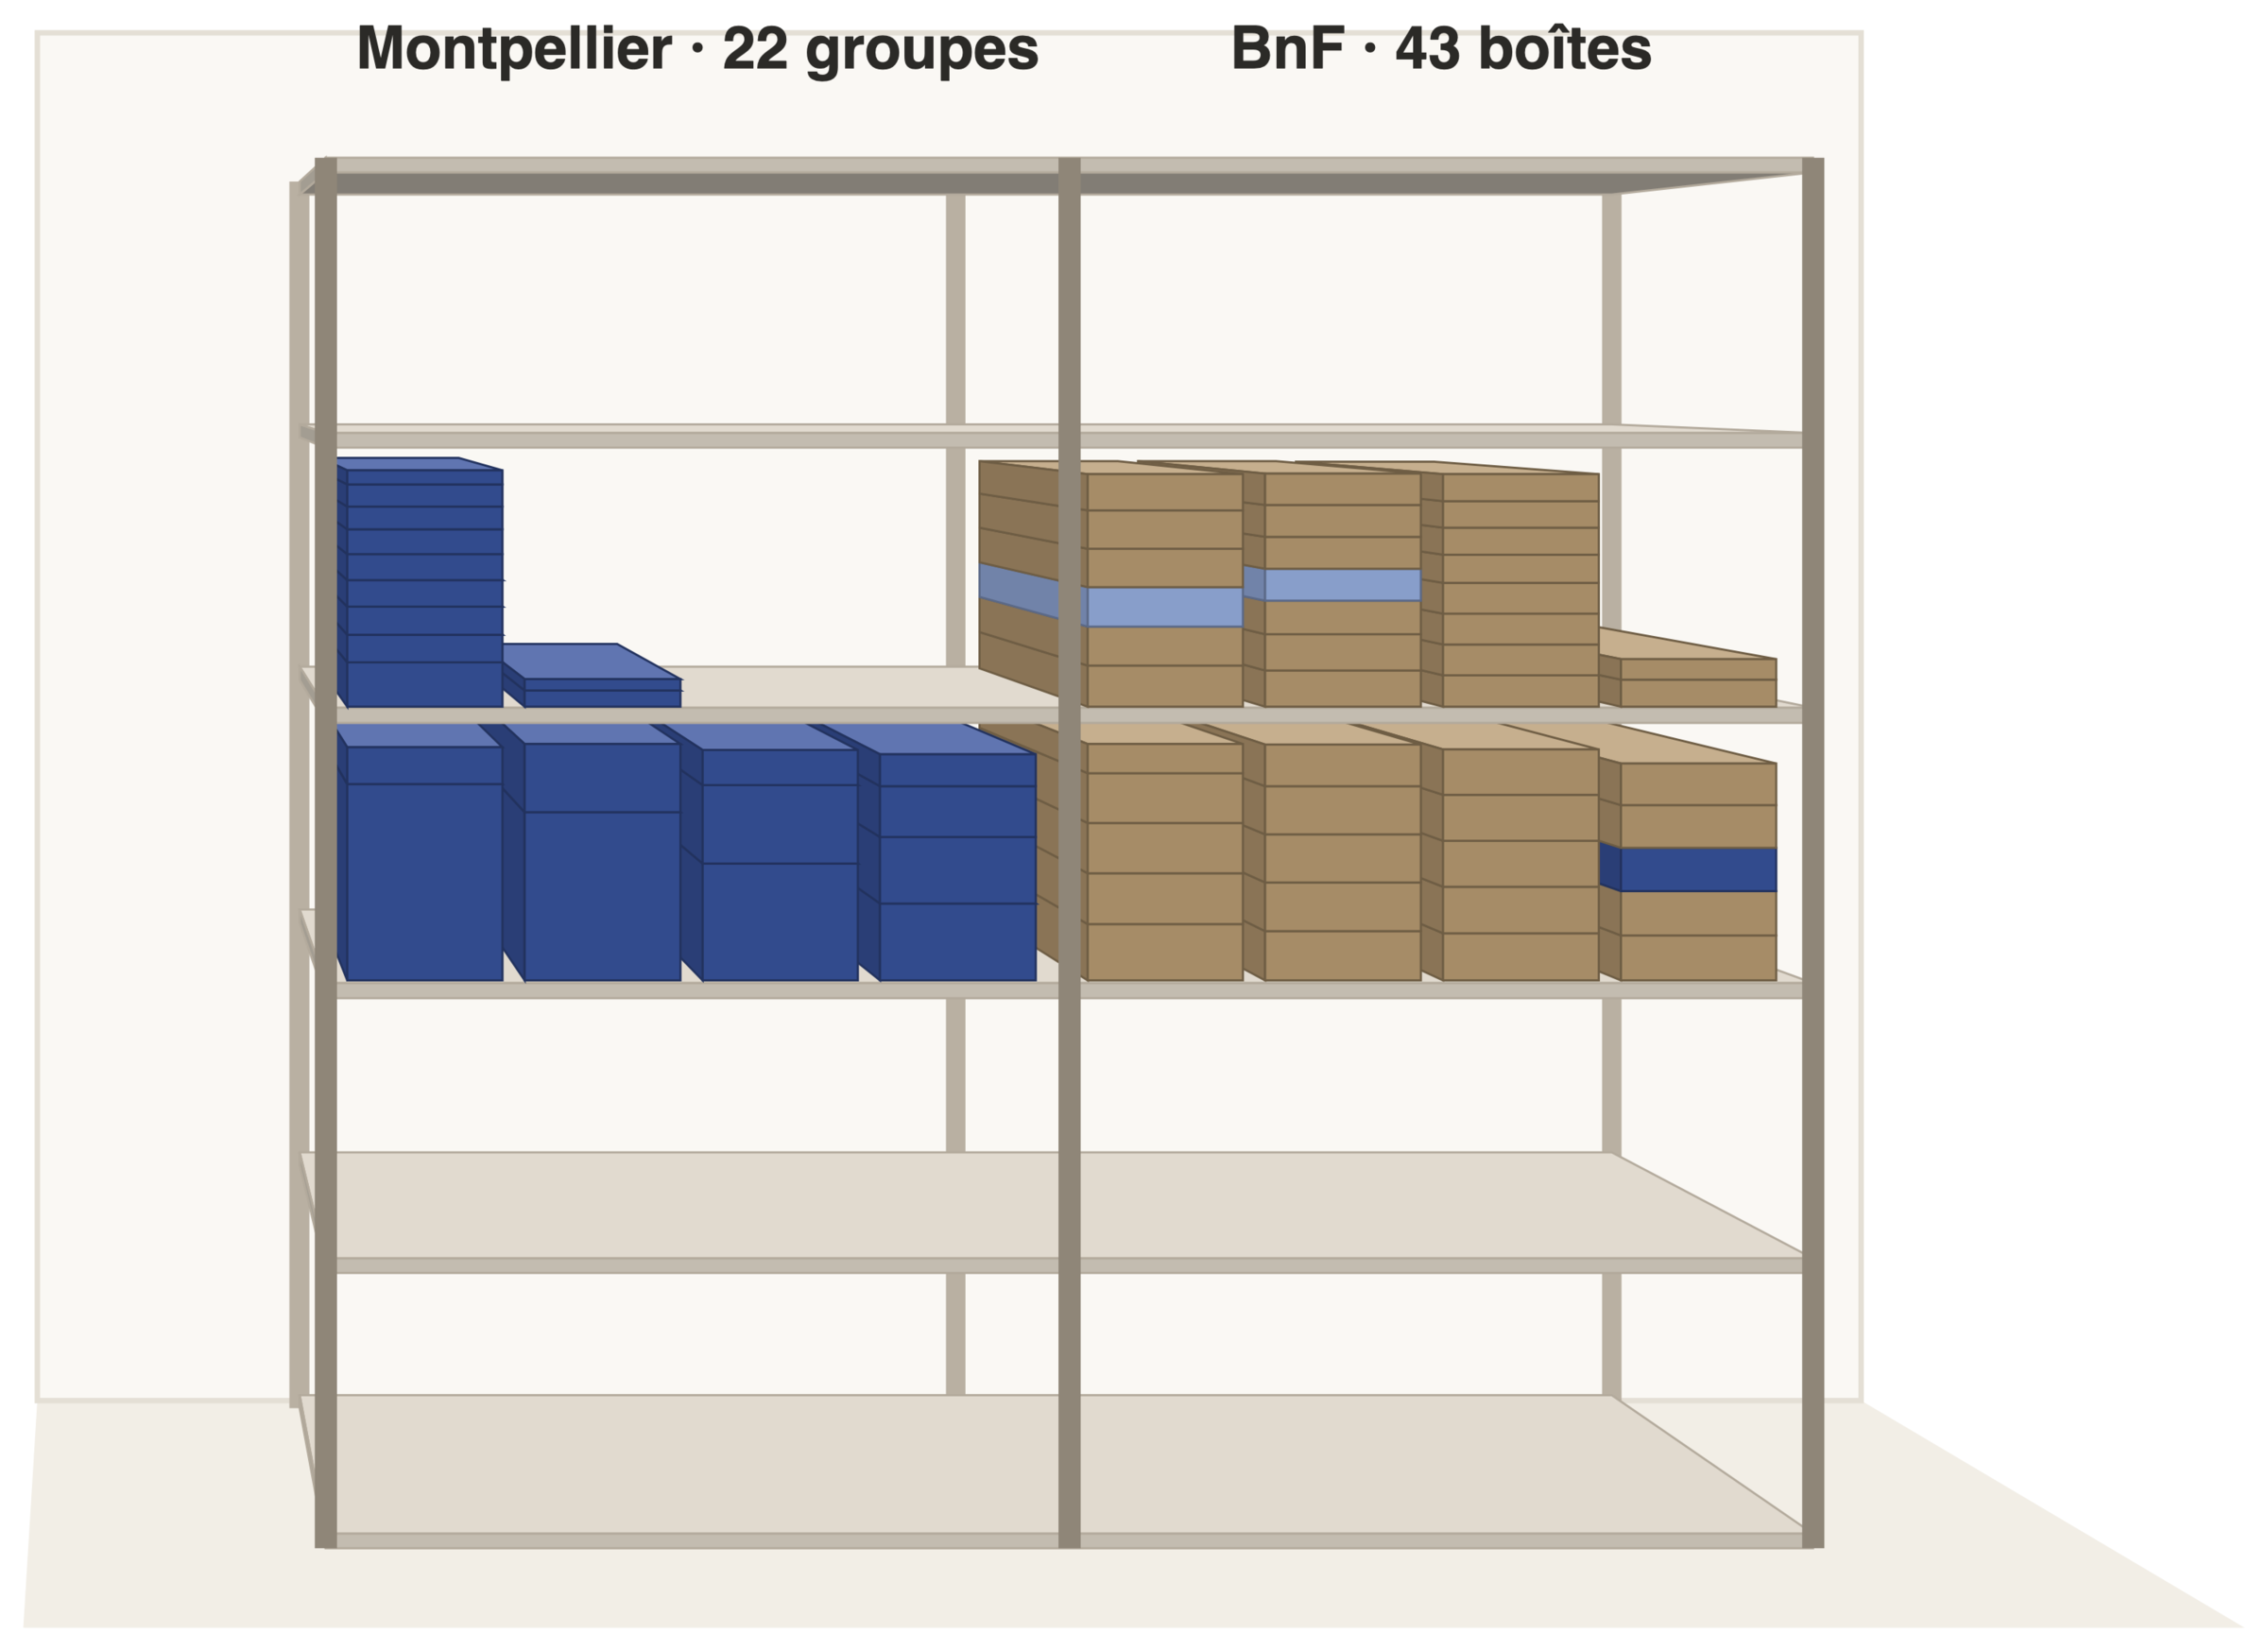
\includegraphics[width=0.9\textwidth]{fig/etageres.png}\par\vspace{1mm}
\raggedright\legende{\textbf{Tout tiendrait sur deux étagères.} Les deux fonds rangés dans une même réserve, à hauteur de bras. Chaque carton a le format d'une feuille A4 et la hauteur de sa pile de papier, à un dixième de millimètre la feuille. À gauche, les 22 groupes de dossiers de Montpellier, tous mathématiques ; à droite, les 43 boîtes de la BnF, en bleu clair celles qui contiennent un peu de mathématiques, en bleu foncé la seule qui en soit entièrement faite. Montpellier compte des pages et la BnF des feuillets : une pile de Montpellier peut donc être jusqu'à deux fois trop haute. Le papier seul est représenté, sans les cartons d'archives.}
\end{minipage}\par\vspace{4mm}

\begin{multicols}{3}
\inter{Deux fonds, deux mondes}
Mises côte à côte, les deux collections racontent deux vies. À Montpellier, tout est mathématique, et les plus gros ensembles sont ceux de la maturité : la « Géométrie et topologie combinatoire » (plus de 2\,600 pages) et les \emph{Dérivateurs} (près de 2\,300). À la BnF, il faut chercher la mathématique : une boîte sur quarante-trois, et quelques feuillets dispersés dans trois autres.

Ce déséquilibre a une conséquence pratique. Les chercheurs qui veulent suivre les dernières mathématiques de Grothendieck doivent aller à Paris, consulter des boîtes dont la plupart des pages parlent d'autre chose, avec un crayon à papier et sans photocopieuse. C'est justement ce que préparent les fiches de visite de ce projet : savoir à l'avance dans quelle pochette chercher, et quoi y vérifier.

\begin{encadre}{Comment lire une page de Grothendieck}
Une page typique mêle phrases, formules et schémas. La transcription garde trace de tout ce qui est incertain : un mot \emph{deviné}, un mot \emph{illisible}, un passage \emph{biffé}, un ajout dans la marge. Rien n'est corrigé en silence. La lecture modernisée, elle, peut réécrire, mais chaque écart avec la page est signalé en note. Quand la lecture et la page divergent, c'est la page qui fait foi.
\end{encadre}

\inter{Quatorze énigmes}
Lean ne peut vérifier qu'un énoncé dont les objets existent dans sa bibliothèque, Mathlib. Or Grothendieck travaillait justement là où elle s'arrête : cohomologie étale, champs, topos, motifs. Près d'une centaine d'énoncés restent ainsi hors de portée. Quatorze, parmi les plus précis, ont été rassemblés dans un document à l'intention des mathématiciens, avec pour chacun la page du manuscrit, ce que l'on sait, et ce qui permettrait de trancher.
\end{multicols}
\folio{3}
\newpage

% ------------------------------------------------------------- page 4
\begin{tcolorbox}[colback=papier,colframe=papier,arc=0pt,boxrule=0pt,left=5mm,right=5mm,top=4mm,bottom=4mm]
{\surtitre{Le théorème expliqué}}\par\vspace{1mm}
{\titre\color{encre}\fontsize{22}{25}\selectfont Les droites qui n'en sont pas}\par\vspace{2mm}
{\sans\fontsize{10.5}{14}\selectfont En 1981, Grothendieck s'intéresse à des courbes qui se comportent comme des droites. Il énonce un résultat sans le démontrer. Quarante-cinq ans plus tard, la preuve tient en quelques lignes.}\par\vspace{3mm}
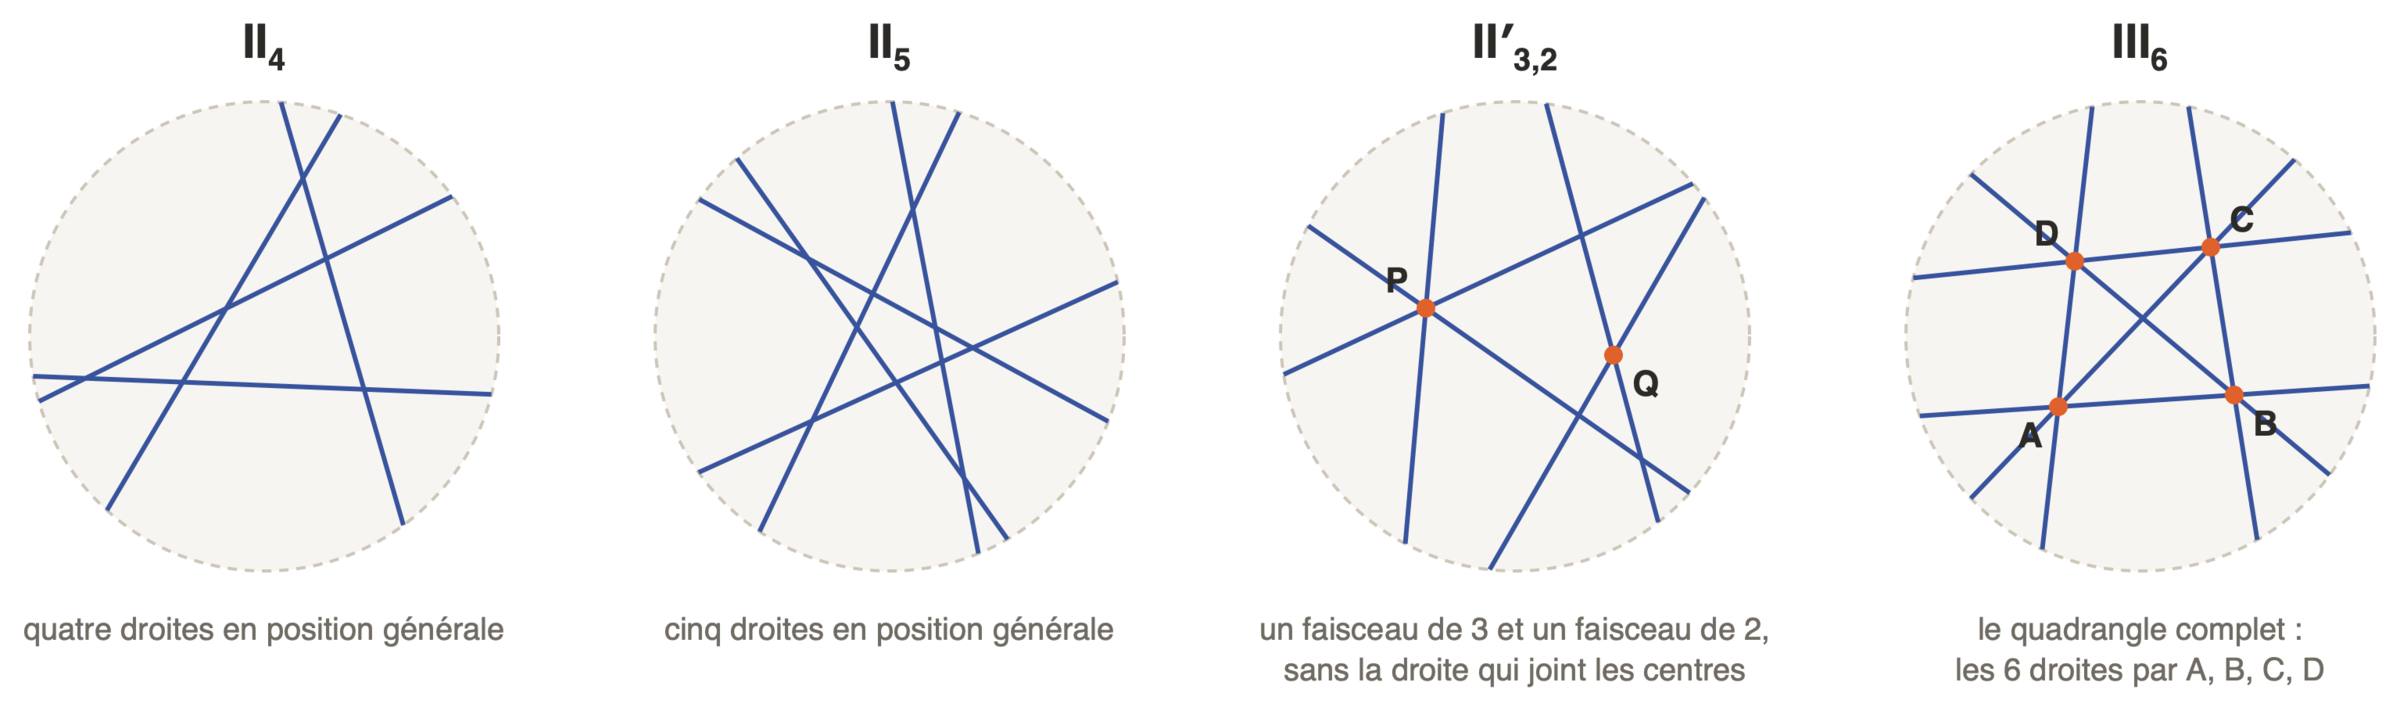
\includegraphics[width=\linewidth]{fig/bigon-configurations-fr.png}\par\vspace{1mm}
\legende{Les quatre dessins de Grothendieck. Dans chacun, toute courbe porte au moins trois croisements. Les points orange marquent les endroits où trois courbes se croisent.}\par\vspace{3mm}
\begin{multicols}{2}
\sans\fontsize{9}{12}\selectfont
Tracez sur une feuille des courbes qui ne sont pas forcément droites, mais qui se croisent deux à deux exactement une fois, comme le feraient des droites. Pour que deux courbes « parallèles » se croisent aussi, on travaille dans le plan projectif, un plan où l'horizon est recollé à lui-même. Ces courbes s'appellent des pseudo-droites.

Grothendieck s'intéresse aux dessins où chaque courbe porte au moins trois points de croisement. Il affirme qu'un tel dessin est soit fait de quatre courbes en position générale, soit contient l'un des trois motifs ci-dessus : cinq courbes en position générale, un faisceau de trois et un faisceau de deux, ou le quadrangle complet, les six droites qui passent par quatre points. Mais la démonstration qu'il en donne s'appuie sur un autre énoncé de la même page, qui est faux.

\textbf{La preuve.} Un résultat classique, posé par Sylvester en 1893 et démontré au XX\textsuperscript{e} siècle, valable aussi pour les pseudo-droites, garantit qu'il existe un point où ne se croisent que deux courbes. En partant de ce point, on trouve quatre courbes dont trois ne passent jamais par un même point. Une cinquième courbe passe alors par zéro, un ou deux de leurs six croisements. Zéro : on obtient cinq courbes en position générale. Un : le faisceau de trois et de deux. Deux : la courbe est forcément une « diagonale ». Une diagonale seule ne porterait que deux croisements, ce qui est interdit ; deux diagonales forment le quadrangle complet. Le théorème est démontré.

Cette preuve a été écrite par l'édition et vérifiée par ordinateur dans un modèle combinatoire des dessins. Aucun spécialiste ne l'a encore relue. La question suivante de Grothendieck, savoir si le squelette d'un tel dessin suffit à le reconstituer, est démontrée quand aucun point ne réunit plus de deux courbes, et reste ouverte dans les autres cas.
\end{multicols}
\end{tcolorbox}

\vspace{3mm}
\begin{multicols}{3}
\inter{Ce que la machine ne sait pas faire}
La machine lit vite, mais elle est très sûre d'elle, même quand elle se trompe : il lui arrive de croire ouverte une question réglée depuis longtemps, ou de prêter à un livre un résultat qu'il ne contient pas. C'est pourquoi chaque lecture douteuse est signalée, chaque argument de l'édition marqué comme tel, et chaque énoncé confronté à la page.

\inter{Et maintenant}
Le projet continue : transcrire les derniers dossiers, vérifier sur les fac-similés les lectures douteuses, et retourner à la BnF pour mesurer ce que contiennent les boîtes mathématiques. Surtout, il faut que des mathématiciens s'emparent de ces pages. Grothendieck écrivait pour lui-même ; quarante ans plus tard, ses brouillons attendent toujours leurs lecteurs.

\vspace{2mm}
\begin{encadre}{Pour aller plus loin}
Les fac-similés du fonds de Montpellier sont en libre accès sur le site de l'université : grothendieck.umontpellier.fr. Les notices du fonds de la BnF (NAF 29093) sont consultables sur archivesetmanuscrits.bnf.fr. Pour les topos, la grande idée des années 1960, on peut lire Jean Malgoire, « Un héritage mathématique fertile », \emph{Pour la Science}, n\textsuperscript{o}~467, septembre 2016 : c'est à lui que Grothendieck a confié ses manuscrits.
\end{encadre}
\end{multicols}
\folio{4}

\end{document}
